\documentclass[a4paper,11pt]{article}

\usepackage{polyglossia}
\setdefaultlanguage{latvian}

\usepackage{graphicx}
\usepackage{placeins}
\usepackage{fixlatvian}



\begin{document}

\author{Jānis Ratnieks (jr09103)}
\title{Datoru tīkli }
%\subtitle{1. mājas darbs}

\date{\today}

\maketitle
\begin{center}
1. mājas darbs
\end{center}






\section{ uzd.}

Ieejošais signāls, skatīt attēlus \ref{fig1} un \ref{fig2}, sastādīts no attiecīgi 20 un 10 harmonikām (atsevišķās harmonikas arī redzamas attēlos). Aprēķinu rezultāti koeficientiem $a_n, b_n$ un $c$ redzami zemāk. Skaitliskās vērtības pārējiem koeficientiem aprēķinātas ar \textit{python numpy} bibliotēkas \textit{fft} funkciju un apskatāmas tabulās. Pielikumā parādīts pilns python kods attēlu un koeficientu ģenerēšanai. Kods nav labākais kodēšanas piemērs, tomēr ātrākais, lai tiktu pie rezultāta, vismaz manā gadījumā.

$$c=\frac{2}{T}\int_{0}^{1}g(t)dt -> 2\cdot 0.5=1$$
$$a_{n}=\frac{2}{T}\int_{0}^{T}g(t)cos(2 \pi ntf)dt =$$
(trīs gadījumos $g(t)=0$, bet pārējos $g(t)=1$ un izteiksmi var sadalīt divos integrāļos. Pieņemot, ka $f=1$.)
$$= 2(\int_{\frac{1}{8}}^{\frac{1}{4}}cos(2\pi nt)dt+\int_{\frac{1}{2}}^{\frac{7}{8}}cos(2\pi nt)dt)$$
$$a_1= 2(\int_{\frac{1}{8}}^{\frac{1}{4}}cos(2\pi t)dt+\int_{\frac{1}{2}}^{\frac{7}{8}}cos(2\pi t)dt)=\frac{1}{\pi}(\left.(sin(2\pi t))\right\vert_{\frac{1}{8}}^\frac{1}{4}+\left.(sin(2\pi t))\right\vert_{\frac{1}{2}}^\frac{7}{8})$$


$$=\frac{1}{\pi}(sin(\frac{\pi}{2})-sin(\frac{\pi}{4})+sin(\frac{7\pi}{4})-sin(\pi))=\frac{1}{\pi}(1-\frac{\sqrt{2}}{2}-\frac{\sqrt{2}}{2})=\frac{1}{\pi}(1-\sqrt{2})$$

$$a_2= 2(\int_{\frac{1}{8}}^{\frac{1}{4}}cos(4\pi t)dt+\int_{\frac{1}{2}}^{\frac{7}{8}}cos(4\pi t)dt)=\frac{1}{2\pi}(sin(\pi)-sin(\frac{\pi}{2})+sin(\frac{7\pi}{2})-sin(2\pi))=$$
$$=\frac{1}{2\pi}(-1-1)=-\frac{1}{\pi}$$

Aprēķinātie $a_n$:
\begin{table}[]
\begin{tabular}{|l|l|l|l|l|l|l|l|l|l|}
\cline{1-10}
$a_1$ &$a_{2}$  &$a_3$  &$a_4$  &$a_5$  &$a_6$  &$a_7$  &$a_8$  &$a_9$  &$a_{10}$  \\ \cline{1-10}
 -0.132 & -0.318 & -0.256 & 0 & 0.154 & 0.106 & 0.0187 & 0 & -0.0147 & -0.063 \\ \cline{1-10}
\end{tabular}
\end{table}

Aprēķini $b_n$ ir ļoti līdzīgi $a_n$ aprēķiniem, tādēļ parādīts tikai $b_1$ aprēķins.

$$b_n = \frac{2}{T}\int_{0}^{T}g(t)sin(2\pi nft)dt=2(\int_{\frac{1}{8}}^\frac{1}{4}sin(2\pi nft)+\int_{\frac{1}{2}}^\frac{7}{8}sin(2\pi nft)dt)$$
(Līdzīgi kā iepriekš $f=1$ un $T=1$, bet $g(t)=1$ apgabalos, kur $V=1$ un $g(t)=0$, kur $V=0$.
$$b_1 = 2(\int_{\frac{1}{8}}^\frac{1}{4}sin(2\pi t)+\int_{\frac{1}{2}}^\frac{7}{8}sin(2\pi t)dt)=$$
$$=\frac{1}{\pi}(\left.(cos(\frac{\pi}{2}t)-cos(\frac{\pi}{4}t))\right\vert_{\frac{1}{8}}^\frac{1}{4} +\left.(cos(\frac{7\pi}{4}t)-cos(\pi t))\right\vert_{\frac{1}{2}}^\frac{7}{8})=$$
$$=\frac{1}{\pi}(0-\frac{\sqrt{2}}{2}+\frac{\sqrt{2}}{2}+1=\frac{1}{\pi}$$

Apreķinātie $b_n$ redzami tabulā:

\begin{table}[!h]
\begin{tabular}{|l|l|l|l|l|l|l|l|l|l}
\cline{1-10}
$b_1$ &$b_2$  &$b_3$  &$b_4$  &$b_5$  &$b_6$  &$b_7$  &$b_8$  &$b_9$  &$b_{10}$  \\ \cline{1-10}
 0.318 & -0.318 & 0.105 & 0 & 0.064 & -0.106 & 0.046 & 0 & 0.035 & -0.064 \\ \cline{1-10}
\end{tabular}
\end{table}

\begin{figure}
\centering
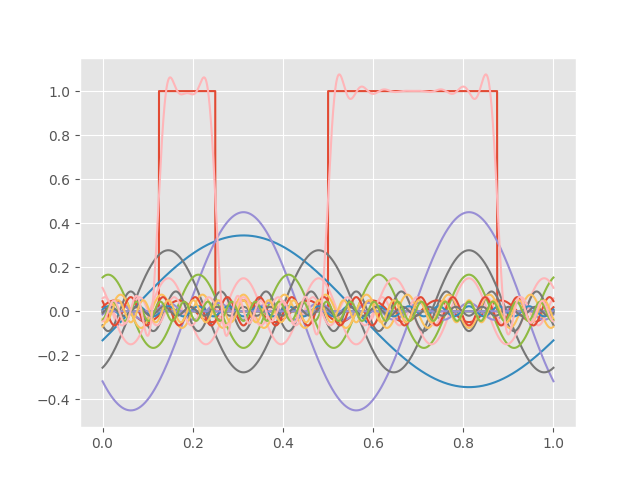
\includegraphics[scale=0.7]{Fig1.png}
\caption{Modulējamais signāls, reālais signāls un atsevišķās harmonikas 20 koeficientu pāriem.}
\label{fig1}
\end{figure}

\begin{figure}
\centering
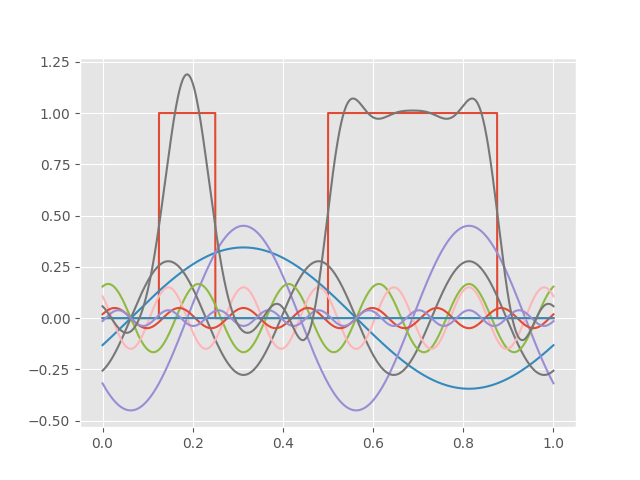
\includegraphics[scale=0.7]{Fig10x.png}
\caption{Modulējamais signāls, reālais signāls un atsevišķās harmonikas 20 koeficientu pāriem.}
\label{fig2}
\end{figure}


\FloatBarrier
\section{ uzd.}
MDR=max data rate
\begin{equation}
MDR_{Nyquist}=2Hlog_2V \frac{bit}{sec}
MDR_{Nyquist}=2\cdot 3e3\cdot log_24=12 \frac{kbit}{sec}
\end{equation}

\begin{equation}
MDR_{Shannon}=Hlog_2(1+S/N)
MDR_{Shannon}=3e3log_2(101)=3\cdot 6.66e3=20 \frac{kbit}{sec}
\end{equation}

Šajā gadījumā, lai pateiktu, kurš no vienādojumiem norādīs uz datu pārneses apjomu jāsaprot, kurš vienādojums ko aprēķina. Nyquist vienādojums apreķina maksimālo datu pārraides apjomu dotam pārraides līmeņu skaitam, bet Shannon risinājums ir atvasināts no informācijas entropijas teorijas, kuru viņš pats arī izveidoja. Informācijas entropija skatās uz to, cik daudz informācijas var nosūtīt, neatkarīgi no kanālu skaita. Ja Šenona entropija būs maksimāla, kas atbilst pilnīgam troksnim jeb bezgalīgi lielam kanālu saitam, tad $S/N->0$, jo $N->\infty$. Šajā gadījumā ir skaidrs, ka pieņemtais kanālu skaits pirmajam aprēķinam ar Nyquist formulu ir nepietiekams un teorētiski iespējams nosūtīt vairāk informācijas, palielinot kanālu skaitu. Tādēļ jāņem vērā Šenona vienādojums, ja grib zināt maksimāli iespējamo datu nosūtīšanas apjomu.

\section{ uzd.}
CDMA signāls redzmas tabulā \ref{tabcdma} un apzīmēts ar S burtu, tā ir superpozīcija no visiem pārējiem signāliem. Tā kā atslēgas A, B, C un D ir savsarpēji ortogonālas, $A\cdot B=0$, tad viennozīmīgi iespējams atkodēt signālu. To dara reizinot S ar katru no atslēgām un izdalot ar signāla garumu, reizinājumi atzīmēti tabulā \ref{tabcdma} ar apzīmējumu $\Pi _XY$. Pēc tam izdala ar kopējo signāla garumu jeb šajā gadījumā 8 un iegūst rezultātu. Atkarībā no notācijas -1 var apzīmēt vai nu 1 vai 0 un 1 attiecīgi 0 vai 1. Ja summa ir 0, tad dotais raidītājs attiecīgajā brīdī neraida, kā tas ir A gadījumā.
\begin{table}[]
\begin{tabular}{|l|l|l|l|l|l|l|l|l|l|}
\hline
S&-1&3&-3&1&-1&-1&-1&-1&  \\ \hline
A&-1&-1&-1&1&1&-1&1&1&   \\ \hline
$\Pi_{AS}$&1&-3&3&1&-1&1&-1&-1& =>0\\ \hline
B&-1&-1&1&-1&1&1&1&-1& \\ \hline
$\Pi_{BS}$&1&-3&-3&-1&-1&-1&-1&1&=>-1 \\ \hline
C&-1&1&-1&1&1&1&-1&-1& \\ \hline
$\Pi_{CS}$&1&3&3&1&-1&-1&1&1&=>1 \\ \hline
D&-1&1&-1&-1&-1&-1&1&-1& \\ \hline
$\Pi_{DS}$&1&3&3&-1&1&1&-1&1&=>1 \\ \hline
                     
\end{tabular}
\caption{CDMA signālu atšifrēšana.}
\label{tabcdma}
\end{table}

\FloatBarrier

\section{ uzd.}
Kā redzmas attēlos \ref{bin} un \ref{quad}, tad pirmajā fāzes maiņa notiek pie katras 1 un 0 maiņas, bet otrais gadījums sadalīts 4 daļās, jo spēj pārraidīt pārus "00", "01", "10" un "11".
\begin{figure}[!h]

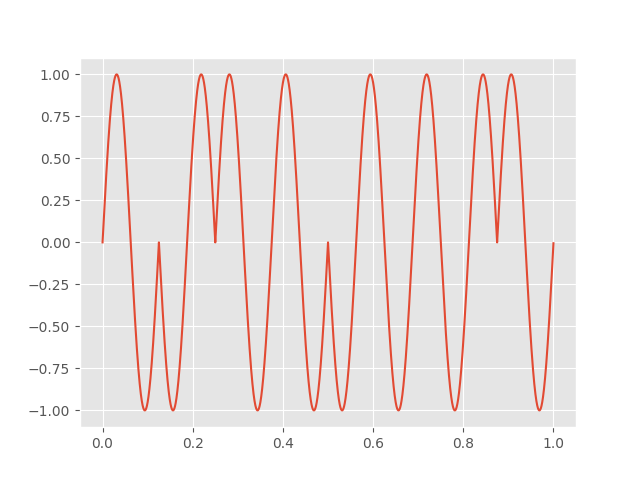
\includegraphics[scale=0.8]{bpsk.png}
\caption{Binary Phase Shift Keying}
\label{bin}
\end{figure}

\begin{figure}[!h]

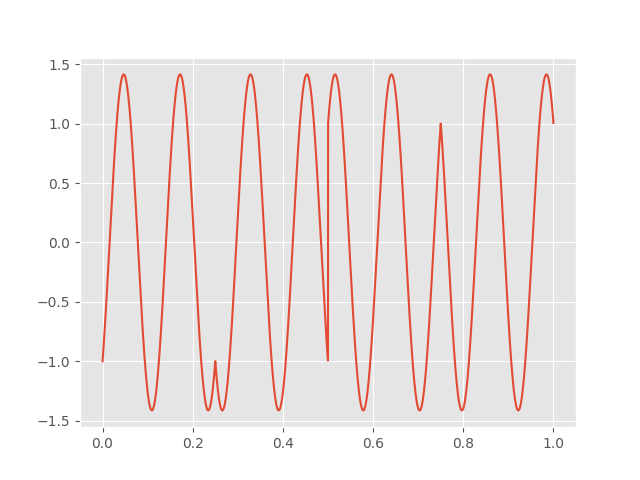
\includegraphics[scale=0.8]{qpsk.png}
\caption{Quadrature Phase Shift Keying}
\end{figure}
\label{quad}

\pagebreak
\pagebreak
\section*{Pielikums}

\begin{verbatim}
import numpy as np
import matplotlib.pyplot as plt
from matplotlib.pyplot import style

style.use('dark_background')

########### A #################
# 01010100
telpa=np.arange(0,1,0.0001)
xs=np.array([])
for i in range(len(telpa)):
    if i<1250:
        xs=np.append(xs,0)
    elif i<2500:
        xs=np.append(xs,1)
    elif i<5000:
        xs=np.append(xs,0)
    elif i<8750:
        xs=np.append(xs,1)
    else:
        xs=np.append(xs,0)
Is=np.array([])
Qs=np.array([])
for i in range(len(telpa)):
    if i<2500:
        Is=np.append(Is,-1)
        Qs=np.append(Qs,1)
    elif i<5000:
        Is=np.append(Is,-1)
        Qs=np.append(Qs,-1)
    elif i<7500:
        Is=np.append(Is,1)
        Qs=np.append(Qs,1)
    else:
        Is=np.append(Is,1)
        Qs=np.append(Qs,-1)


plt.plot(telpa, xs)
#Do a fourier transform

a=np.fft.fft(xs)

an=np.array(np.real(a[1:10]/5000))
bn=np.array(np.imag(a[1:10]/5000))
summa=np.zeros(10000)
for i in range(len(an)):
    #plt.plot(telpa, an[i]*np.cos(2*np.pi*(i+1)*telpa)+bn[i]*np.sin(2*np.pi*(i+1)*telpa))
    summa=summa+an[i]*np.cos(2*np.pi*(i+1)*telpa)-bn[i]*np.sin(2*np.pi*(i+1)*telpa)

plt.plot(telpa,summa+0.5)
plt.show()

for i in range(len(an)):
    print(','.join(str(a[i]) for i in range(len(an))))


print(an)
print(bn)


plt.plot(np.sqrt(np.real(a[0:10])**2+np.imag(a[0:10])**2),linewidth=0, marker='*')
plt.show()

######### B ###########

'''
A. (Obligātā daļa uz 7) Patstāvīgi atkārtot gramatā 2.1.1 nodaļā ilustrēto Furje transformāciju, tikai parraidāmā baita vietā ņemt ASCII kodu lielajam burtam, kas sakrīt ar Jūsu vārda trešo burtu (bez garumzīmēm, mīkstinājuma zīmēm). Aprēķināt vismaz pirmās 10 harmonikas un rezultātus attēlot arī grafiski, lai grafiski novērotu sākotnējā signāla pakāpenisku aproksimāciju. (Furje transformāciju skaitliskās vētības visērtāk rēķnāt un grafiski attēlot MS Excel, Mathematica vai tml. vidē)

B. Četru līmeņu digitāls signāls tiek raidīts caur 3 KHz kanalu, kura trokšņu līmenis ir 20dB. Ar Nikvista un Šenona formulām novērtējiet maksimālo datu parraides ātrumu un izvērtējiet kuras formulas rezultāts šajā gadījumā būtu jēņem vērā novērtējot maksimālo iespējamo datu pārraides ātrumu.

C. CDMA uztvērējs uztvēris sekojošu "čipu" virknīti: (-1 +3 -3 +1 -1 -1 -1 -1). Izmantojot attēlā 2-45(b) definētās raidstacijas un to čipu virknites, noskaidrot kuras no raidstacijam A,B,C,D ir raidījušas un kādu bitu (0 vai 1) katra no raidošajām stacijām ir noraidījusi?

D. (Neobligata dala uz 10) Grafiski uzkonstruējiet signāla formu (dažus periodus), kas caur 0-4KHz frekvenču joslu ļautu parraidīt datus ar ātrumu 8Kbps. Pamatojiet, kāpēc jūsu uzkonstruētajam signālam nav būtisku harmoniku augstāku par 4KHz. Kas būtu jāizmaina, lai jūsu uzkonstruēto signālu pārvērstu ierobežotas frekvenču josas radio-signālā (piemēram 100-104KHz)?


'''

bpsk=np.sin(2*np.pi*8*telpa+xs*np.pi)
plt.plot(telpa, bpsk)
plt.show()


I=Is*np.cos(2*np.pi*8*telpa)
Q=Qs*np.sin(2*np.pi*8*telpa)

plt.plot(telpa, (I+Q))
plt.show()






\end{verbatim}


\end{document}